\begin{frame}{User Activeness}
    \begin{enumerate}
        \item New criteria used as a component of Reward along with traditional click information
        \item Activeness of user is modeled using Survival models (cite here)
        \begin{equation}
            S(t) = e^{- \int_0^t \lambda(x)dx}
        \end{equation}
        \item $\lambda(t) = \lambda_0$ is set as the constant probability of click happening after time t
        \item Every time a click happens user activeness is incremented as $S(t) = S(t) + S_a$
        \item Total Reward : $r_{total} = r_{click} + r_{active}$
        \begin{figure}
            \centering
            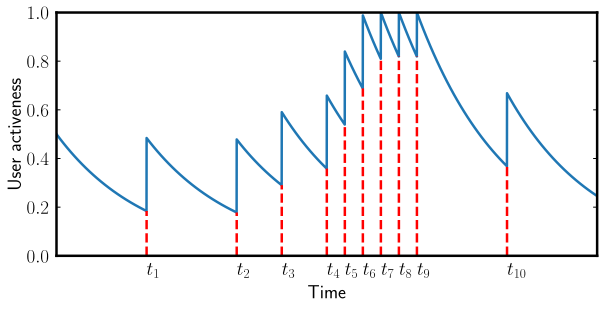
\includegraphics[scale=0.3]{DeepinScreenshot_select-area_20200514225125.png}
            %\caption{}
            \label{fig:user_activeness}
        \end{figure}
    \end{enumerate}
\end{frame}



\begin{frame}{Exploration}
\begin{columns}
\begin{column}{0.7\textwidth}
   \begin{enumerate}
       \item Dueling Bandit Gradient Descent (DBGD) is used to do exploration
       \item Two Q networks, $\Tilde{Q}$ is a perturbation of $Q$
       \item $\Tilde{W} = W + \alpha \cdot rand(-1,1) \cdot W$
       \item Recommended lists $L$ and $\Tilde{L}$ are merged into $\hat{L}$ via probabilistic interleaving
       \item If item recommended by $\Tilde{Q}$ receives better feedback update $Q$ towards $\Tilde{Q}$
       \item $W^* = W + \eta\Tilde{W}$
       \item Otherwise $Q$ is unchanged
   \end{enumerate}
\end{column}
\begin{column}{0.3\textwidth} 
    \begin{center}
     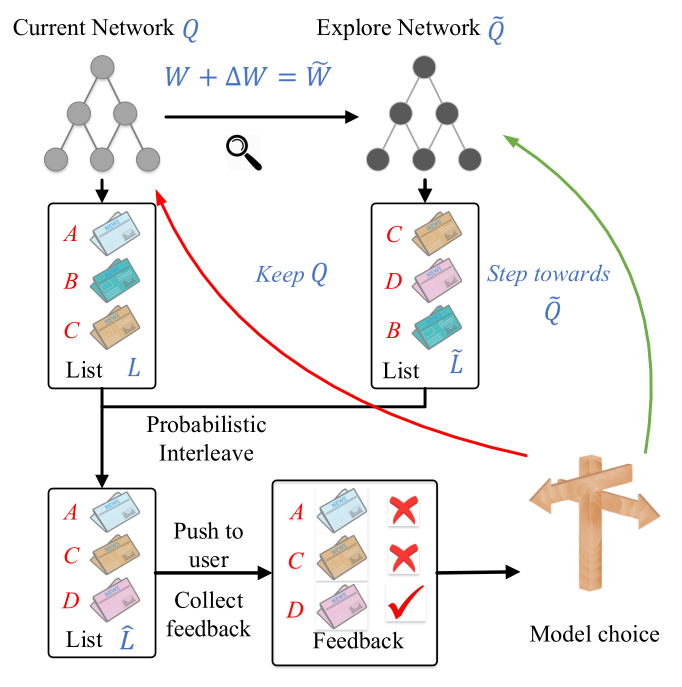
\includegraphics[scale=0.2]{DeepinScreenshot_select-area_20200514225903.png}
     \end{center}
\end{column}
\end{columns}
\end{frame}


\begin{frame}{Evaluation Measures}
    \begin{enumerate}
        \item Click Through Rate (CTR)
        \begin{equation}
            CTR = \frac{number\, of\, clicked\, items}{number\, of\, total\, items}
        \end{equation}
        \item Precision at k
        \begin{equation}
            Precision@k = \frac{number\, of\, clicks\, in\, top\, k\, recommended\, items}{k}
        \end{equation}

    \item Normalized Discounted Cumulative Gain (nDCG)
    \begin{equation}
        DCG(f) = \sum\limits_{r=1}^n y_r^f \frac{1}{log(1+r)}
    \end{equation}
    \end{enumerate}
\end{frame}